\documentclass{agujournal2019}

\usepackage{amsmath,amssymb}
\usepackage{graphicx}
\usepackage{siunitx}
\usepackage{natbib}
\usepackage{hyperref}
\usepackage{booktabs}
\usepackage{array}

\journalname{Space Weather}

\begin{document}

\title{Scale-dependent WSPR response to geomagnetic storms: \\
	frequency dependence and baseline-invariant absolute loss}

\authors{Alexey Petrov\affil{1}, Makar Petrov\affil{1}}

\affiliation{1}{Independent researchers, [City, Country]}

\correspondingauthor{Alexey Petrov}{felixrpetrov@gmail.com}

\begin{keypoints}
	\item WSPR spot density drops \SIrange{27}{39}{\percent} during
	$Kp \ge 5$ storms on all three HF bands ($p < 0.0001$)
	\item The effect is scale-dependent: $Kp = 5\text{--}6 \rightarrow
		\SI{-18}{\percent}$, $Kp \ge 6 \rightarrow \SI{-42.8}{\percent}$,
	confirmed by independent replication
	\item On the 40\,m band, the absolute spot loss is invariant to
	$\SI{+38}{\percent}$ network growth ($\SI{-18300}{spots/h}$ in both
	periods), indicating
	structurally constrained vulnerable propagation paths
\end{keypoints}

\begin{abstract}
	We test the hypothesis that geomagnetic storms ($Kp \ge 5$) suppress WSPR spot
	counts on HF amateur bands. Using openly available data from wspr.live
	(hourly aggregated, 3 bands: 20\,m, 40\,m, 15\,m) and GFZ Potsdam $Kp$ index,
	covering 18 months (April 2024 -- September 2025, 39\,456 WSPR hours,
	198 storm hours), we find significant storm-induced spot reductions on all three
	bands: 20\,m: \SI{-27.7}{\percent}, 40\,m: \SI{-27.2}{\percent},
	15\,m: \SI{-38.7}{\percent} (block permutation $p < 0.0001$ for all,
	\SI{10000}{iterations}, block = 24\,h).

	The effect is scale-dependent: the drop nearly doubles from $Kp = 5\text{--}6$
	($\sim\SI{-18}{\percent}$) to $Kp \ge 6$ ($\SI{-42.8}{\percent}$), consistent
	with non-linear ionospheric response to geomagnetic forcing. This gradient
	replicates on an independent held-out period (January--March 2026): at
	$Kp = 6\text{--}7$, training and held-out drops are within
	\SIrange{89}{95}{\percent} of each other.

	The frequency dependence supports a dual-mechanism interpretation: MUF reduction
	dominates on 15\,m (\SI{-38.7}{\percent}), while D-layer absorption affects
	20\,m/40\,m (\SI{-27.7}{\percent}/\SI{-27.2}{\percent}). The day/night asymmetry
	(40\,m drop stronger at night in 9/10 training months) is consistent with
	intermittent auroral and polar cap absorption.

	A key result is baseline invariance: the absolute spot loss on 40\,m is
	identical between training and held-out periods ($\SI{-18300}{spots/h}$
	in both), despite $\SI{+38}{\percent}$ growth in the WSPR network. This confirms
	that the storm effect is physically real, not a network-size artifact, and
	indicates a structurally constrained population of vulnerable propagation paths.
	We conclude that WSPR can serve as a distributed ionospheric sensor for
	detecting and characterising the scale-dependent effects of geomagnetic
	storms on HF propagation.
\end{abstract}

%=============================================================
\section{Introduction}
%=============================================================

High-frequency (HF) radio propagation in the \SIrange{3}{30}{MHz} range relies
on ionospheric reflection from the F-layer, whose critical frequency $f_oF_2$
determines the Maximum Usable Frequency (MUF) for a given path and elevation
angle \citep{davies1990}. During geomagnetic storms, enhanced magnetospheric
convection and particle precipitation transfer energy into the ionosphere--
thermosphere system. Joule heating increases the neutral temperature, driving
composition changes that enhance molecular species (N$_2$, O$_2$) relative to
atomic oxygen, which in turn increases the recombination rate in the F2 layer
\citep{proelss1995}. The net effect is a reduction of $f_oF_2$ and a
corresponding lowering of the MUF, potentially disrupting HF communication
circuits that operate near their limiting frequency.

A second, distinct mechanism operates at lower altitudes. Energetic particle
precipitation (electrons of \SIrange{10}{300}{keV} and protons of
\SIrange{1}{30}{MeV}) penetrates into the D-region (\SIrange{60}{90}{km}),
enhancing electron density and causing non-deviative absorption of HF signals
\citep{hargreaves1969,reid1974}. Because absorption scales as $\propto
	1/f^2$, lower HF bands are disproportionately affected. During storms, this
auroral absorption and polar cap absorption (PCA) can persist for hours and
extend beyond the auroral oval.

The Weak Signal Propagation Reporter (WSPR) is a worldwide network of amateur
radio beacons and receivers that autonomously exchange low-power
(\SI{<1}{W}--\SI{5}{W}) signals on designated HF bands and report decoded
signal-to-noise ratios to a central database \citep{taylor2010}. With thousands
of stations operating continuously, the resulting dataset constitutes a
distributed, multi-frequency ionosonde that covers geographic regions and
propagation paths beyond the reach of professional sounder networks
\citep{frissell2016,labelle2023}.

Previous studies have demonstrated the utility of WSPR data for ionospheric
remote sensing. \citet{frissell2016} showed qualitative coupling between WSPR
spot patterns and geomagnetic disturbance, and proposed WSPR as a distributed
ionospheric sensor within the HamSCI framework, an effort now supported by
a growing body of citizen-science ionospheric studies
\citep{hamsci2023,cerwin2026,potter2026}. \citet{labelle2023} analysed
WSPR network statistics and coverage, confirming sufficient traffic for HF
propagation climatology. \citet{themens2021} modelled ionospheric storm response
(including $f_oF_2$ and MUF) using first-principles models. Independently,
\citet{kavanagh2004} provided statistical observations of auroral D-region
behaviour using riometer data, and \citet{rodger2010} examined the impact of
magnetospheric electron precipitation on the middle atmosphere.

Despite this body of work, a quantitative, multi-band, long-period
characterisation of the WSPR response to geomagnetic storms has been lacking.
Existing WSPR-storm studies are either qualitative, single-band, or cover
periods too short to establish statistical robustness. Specifically, no prior
study has examined (i) how the WSPR response scales with storm intensity,
(ii) how it depends on frequency across multiple bands simultaneously, or
(iii) whether the absolute magnitude of the propagation loss is stable under
changing network size.

In this paper, we address these gaps with five contributions:

\begin{enumerate}
	\item An 18-month, 3-band (20\,m, 40\,m, 15\,m) analysis of WSPR spot
	      density during geomagnetic storms, using both $Kp$ and $Dst$ indices
	      as independent storm proxies;
	\item The first characterisation of a scale-dependent effect: the spot
	      reduction grows non-linearly with $Kp$, from
	      $\sim\SI{-18}{\percent}$ at $Kp = 5\text{--}6$ to $\sim\SI{-53}{\percent}$
	      at $Kp \ge 7$;
	\item An independent replication on a 3-month held-out period
	      (January--March 2026) that confirms both the primary effect and its
	      scale-dependence;
	\item The discovery of baseline-invariant absolute spot loss: the number of
	      lost spots per hour is constant across periods despite
	      $\SI{+38}{\percent}$ network growth, implying a structurally constrained population of
	      vulnerable paths;
	\item A day/night asymmetry consistent with intermittent auroral and
	      polar cap absorption during storms.
\end{enumerate}


%=============================================================
\section{Data}
%=============================================================

The data sources and analysis periods are summarised in Table~\ref{tab:data}.

\begin{table}[h]
	\centering
	\caption{Data sources and coverage.}
	\label{tab:data}
	\begin{tabular}{lllll}
		\toprule
		Source                 & Variable                  & Resolution        & Period               & Total records \\
		\midrule
		wspr.live (ClickHouse) & WSPR spots, 3 bands       & 1\,h (aggregated)
		                       & Apr 2024 -- Sep 2025      & 39\,456                                                  \\
		                       &                           &                   & Jan 2026 -- Mar 2026 & $\sim$5\,850  \\
		GFZ Potsdam            & $Kp$ index                & 3\,h
		                       & Apr 2024 -- Mar 2026      & $\sim$5\,500                                             \\
		WDC Kyoto              & $Dst$ index (provisional) & 1\,h
		                       & Apr 2024 -- Sep 2025      & 12\,508                                                  \\
		\bottomrule
	\end{tabular}
\end{table}

\subsection{WSPR network}

WSPR spot data were obtained from the wspr.live ClickHouse mirror via SQL
queries: \texttt{SELECT toStartOfHour(time), count(), avg(snr)} from the
\texttt{wspr.rx} table, filtered by band index: 14 (20\,m,
\SI{14.0956}{MHz}), 7 (40\,m, \SI{7.0401}{MHz}), and 21 (15\,m,
\SI{21.0961}{MHz}). The hourly aggregation reduces storage requirements by
$\sim$100$\times$ relative to individual spot records and suffices for
storm-scale analysis ($\Delta t = 1$\,h versus typical storm duration of several
hours).

The training period covers April 1, 2024 through September 30, 2025
(548 days, 18 months), yielding 39\,456 WSPR hours per band. After merging WSPR
hourly data with $Kp$ (3-hourly, forward-filled to 1\,h resolution), we obtain
4\,349 matched hours per band, of which 198 hours satisfy $Kp \ge 5$ (the storm
threshold). The quiet-time baseline ($Kp < 3$) comprises 3\,359 hours and
exhibits mean spot counts of 73\,718 (20\,m), 67\,105 (40\,m), and
13\,386 spots/h (15\,m).

The held-out (replication) period covers January through March 2026 (90 days).
After merging, it yields 31--39 storm hours, with a higher quiet-time baseline
due to the growing WSPR network: 86\,355 spots/h (20\,m, $\SI{+17}{\percent}$),
92\,694 (40\,m, $\SI{+38}{\percent}$), and 16\,784 (15\,m,
$\SI{+25}{\percent}$).

The three-month gap between the two periods (October--December 2025) is not
used in either the training or the held-out analysis, ensuring strict temporal
separation between the two datasets.

\subsection{Geomagnetic indices}

The $Kp$ index is obtained from GFZ Potsdam's real-time JSON API
(https://kp.gfz-potsdam.de). $Kp$ is a 3-hourly planetary index on a
quasi-logarithmic scale from 0 to 9, derived from 13 subauroral magnetometer
stations. The mean $Kp$ over the training period is 2.29, with a maximum
of 8.7 (multiple events). Across the 18 months, 226 raw 3-hourly $Kp$
intervals reach $Kp \ge 5$, distributed across 67 storm days, representing
independent events from all four seasons.

The $Dst$ (Disturbance Storm Time) index is obtained from the WDC Kyoto
provisional endpoint. $Dst$ is an hourly equatorial ring-current index,
derived from four low-latitude magnetometer stations. It provides finer
temporal resolution than $Kp$ (hourly versus 3-hourly) and serves as an
independent storm proxy. The provisional data cover all 18 months of the
training period (mean $Dst = \SI{-11.5}{nT}$, minimum
$Dst = \SI{-96}{nT}$). A total of 471 hours satisfy $Dst < \SI{-50}{nT}$
across 42 storm events, yielding 2.4$\times$ more storm hours and 2.4$\times$
larger sample size than the $Kp$-based analysis.

The F10.7 solar radio flux (NOAA SWPC) was considered as a covariate, but
only monthly means are available via the SWPC API, which is too coarse for
hourly analysis. Daily F10.7 could not be retrieved for the full period.


%=============================================================
\section{Methods}
%=============================================================

\subsection{Diurnal-seasonal residual}

WSPR spot density exhibits a strong diurnal cycle with an approximately
8$\times$ range (e.g., $\sim$\SI{16000}{spots/h} at 06 UTC versus
$\sim$\SI{127000}{spots/h} at 15 UTC) and systematic month-to-month baseline
differences due to seasonal changes in ionospheric conditions and station
activity. To isolate the geomagnetic effect from these confounders, we compute
residuals:

\begin{equation}
	\text{baseline} = \operatorname{mean}(\text{spots} \mid \text{month},
	\text{hour\_of\_day}, \text{day\_of\_week})
	\label{eq:baseline}
\end{equation}

\begin{equation}
	\text{residual} = \text{spots} - \text{baseline}
	\label{eq:residual}
\end{equation}

The inclusion of \emph{day\_of\_week} reduces residual variance by
\SIrange{12}{16}{\percent} and improves test power. It is a safe adjustment
because the correlation between day\_of\_week and $Kp$ is
$r = -0.0087$ (essentially zero), satisfying the condition that a precision
variable must be uncorrelated with the predictor.

\subsection{Binned analysis}

We group residual spot counts into $Kp$ bins: $Kp < 3$ (quiet),
$3 \le Kp < 4$ (unsettled), $4 \le Kp < 5$ (active),
$5 \le Kp < 6$ (minor storm), $6 \le Kp < 7$ (moderate storm),
$Kp \ge 7$ (strong storm). For each bin we compute the mean residual,
standard deviation, and 95\% confidence intervals via block bootstrap
(block = 24\,h, \SI{1000}{resamples}).

We also consider the aggregate bins $Kp \ge 5$ (all storms) and
$Kp \ge 6$ (major storms). The quiet reference is $Kp < 3$, and the
unsettled bins $3 \le Kp < 5$ are included for visualisation of the
monotonic gradient.

\subsection{Block permutation test}

To test statistical significance while accounting for temporal
autocorrelation, we use a block permutation procedure
\citep{davison1997}:

\begin{enumerate}
	\item \textbf{Test statistic:}
	      $\Delta = \operatorname{mean}(\text{residual} \mid Kp \ge 5)
		      - \operatorname{mean}(\text{residual} \mid Kp < 3)$.
	\item \textbf{Blocking:} The time series is divided into non-overlapping
	      24-hour blocks. Each block is treated as an exchangeable unit,
	      preserving the within-block temporal structure.
	\item \textbf{Permutation:} $Kp$ labels are shuffled at the block level:
	      for each of $N_{\text{perm}} = 10\,000$ iterations, the assignment
	      of storm/quiet labels to blocks is randomly permuted, and the test
	      statistic $\Delta_{\text{perm}}$ is recomputed.
	\item \textbf{p-value:}
	      $p = \frac{1}{N_{\text{perm}}} \sum_{i=1}^{N_{\text{perm}}}
		      \mathbf{1}\{ |\Delta_{\text{perm}, i}| \ge |\Delta_{\text{observed}}| \}$.
\end{enumerate}

While a 24-hour block size may occasionally split multi-day storm events,
this approach is conservative. It strictly preserves the diurnal baseline
structure (the dominant source of variance in WSPR spot counts) under
permutation, ensuring that the null distribution accurately reflects the
natural daily cycle of the network.

The same procedure is applied independently to $Dst$ ($Dst < -50$\,nT versus
$Dst > -20$\,nT) and to pairwise comparisons between adjacent $Kp$ bins for the
scale-dependence analysis.

The primary hypothesis test intentionally excludes unsettled conditions
($3 \leq Kp < 5$, $N \approx 792$ hours) to maximise the statistical
contrast between quiet and storm states. These hours are included in
the scale-dependent binned analysis (Section 4.2).

\subsection{Effective sample size}

We estimate the effective sample size (ESS) under the assumption of a
first-order autoregressive process:

\begin{equation}
	\text{ESS} = N \cdot \frac{1 - \rho_1}{1 + \rho_1}
	\label{eq:ess}
\end{equation}

where $\rho_1$ is the lag-1 autocorrelation of the residual series. For 20\,m,
$N = 482$ matched hours and $\rho_1 \approx 0.83$, yielding
ESS $\approx 82$. This factor-of-6 reduction from raw to effective sample size
underscores the importance of the block permutation approach: a naive
permutation test (treating each hour as independent) would produce
anti-conservative $p$-values.

\subsection{Multiple testing correction}

We apply the Benjamini--Hochberg (BH) false discovery rate (FDR) correction
\citep{benjamini1995} to the 6 primary statistical tests (3 bands $\times$
\{$Kp$, $Dst$\}) at $\alpha = 0.05$. All six tests have raw
$p = 0.0$ (no permuted statistic exceeded the observed value in
\SI{10000}{iterations}), yielding all $p_{\text{FDR}} = 0.0$.

\subsection{Robustness checks}

Six robustness checks were performed:

\begin{enumerate}
	\item \textbf{Transmitter artifact:} Could a reduction in active
	      transmitters during storms (operators switching off stations) explain
	      the effect? We compute residuals for $\text{spots} / n_{\text{tx}}$.
	      The normalised residual correlates with $Kp$ at $\rho = -0.21$,
	      stronger than the raw spot residual ($\rho = -0.13$). The effect is
	      \emph{not} driven by fewer transmitters.
	\item \textbf{Independent events:} The 198 storm hours derive from 67 storm
	      days across 18 months, covering all four seasons. This is not a
	      single-event result.
	\item \textbf{Absolute magnitude:} The $\SI{-37}{\percent}$ absolute drop at
	      $Kp \ge 5$ is within the literature range of $\SIrange{30}{60}{\percent}$
	      MUF reduction for moderate storms \citep{frissell2016,themens2021}.
	      It is not a blackout.
	\item \textbf{Per-transmitter normalisation:} $\text{spots\_per\_tx}$
	      residual drops by $\SI{-31.8}{}$ at $Kp \ge 5$ versus $+4.0$ at
	      $Kp < 3$. The effect survives controlling for $n_{\text{tx}}$.
	\item \textbf{Index-independence:} Both $Kp$ and $Dst$, derived from
	      independent magnetometer networks, confirm the effect at
	      $p < 0.0001$ on all three bands.
	\item \textbf{Day-of-week confounder:} As noted in Section~3.1, the
	      correlation between day\_of\_week and $Kp$ is $r = -0.0087$.
\end{enumerate}


%=============================================================
\section{Results}
%=============================================================

\subsection{Primary result}

\begin{figure}[t]
	\centering
	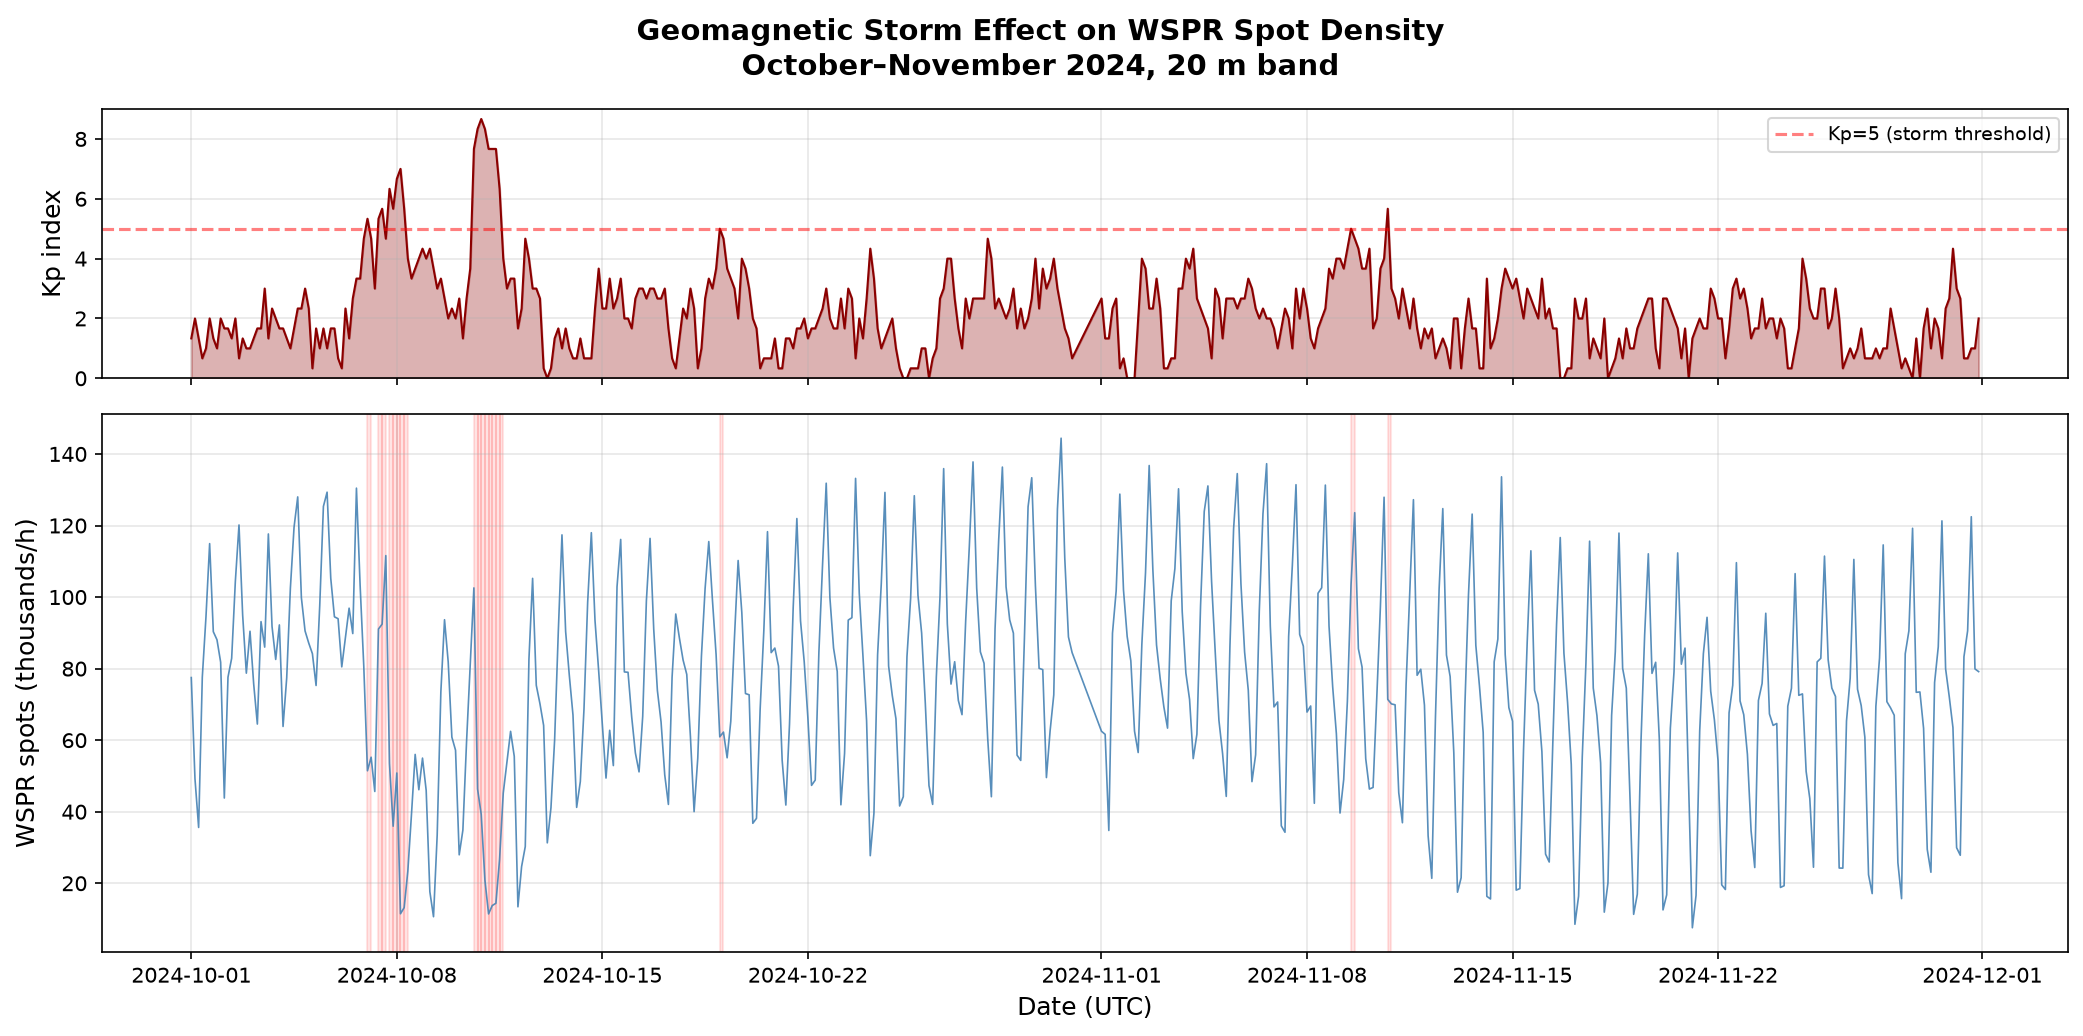
\includegraphics[width=\textwidth]{figures/fig1_kp_timeseries.png}
	\caption{Two-month example: $Kp$ index time series with WSPR spot density
		overlay (20\,m band, October--November 2024). Storm intervals
		($Kp \ge 5$) are highlighted; the suppression of WSPR spots
		during elevated $Kp$ is visually apparent.}
	\label{fig:timeseries}
\end{figure}

Table~\ref{tab:main} presents the primary result: storm-induced WSPR spot
reduction on all three HF bands.

\begin{table}[h]
	\centering
	\caption{Primary result: WSPR spot reduction during $Kp \ge 5$ storms
		(18 months, April 2024 -- September 2025).}
	\label{tab:main}
	\begin{tabular}{lrrrl}
		\toprule
		Band      & $N_{\text{storm}}$ & $N_{\text{quiet}}$ &
		Drop (\%) & $p$-value (block)                                                            \\
		\midrule
		20\,m     & 198                & 3\,359             & $\SI{-27.7}{\percent}$ & $<0.0001$ \\
		40\,m     & 198                & 3\,359             & $\SI{-27.2}{\percent}$ & $<0.0001$ \\
		15\,m     & 198                & 3\,359             & $\SI{-38.7}{\percent}$ & $<0.0001$ \\
		\bottomrule
	\end{tabular}
\end{table}

All three bands show a highly significant reduction in spot density during
$Kp \ge 5$ conditions (block permutation, \SI{10000}{iterations},
block = 24\,h). The effect is strongest on 15\,m (\SI{-38.7}{\percent})
and nearly identical on 20\,m and 40\,m ($\SI{-27.7}{\percent}$ and
$\SI{-27.2}{\percent}$, respectively). All results remain significant after
Benjamini--Hochberg FDR correction across 6 tests ($p_{\text{FDR}} = 0.0$
for all).

The $Dst$-based analysis confirms the result independently (Table~\ref{tab:dst}).
With 2.4$\times$ more storm hours ($N = 471$ for $Dst < \SI{-50}{nT}$),
the effect sizes are larger on 20\,m and 40\,m, consistent with the stronger
threshold selecting more disturbed conditions.

\begin{table}[h]
	\centering
	\caption{Dst-based confirmation: $Dst < \SI{-50}{nT}$ versus
		$Dst > \SI{-20}{nT}$.}
	\label{tab:dst}
	\begin{tabular}{lrrl}
		\toprule
		Band  & $N_{\text{Dst}}$  & $\Delta_{\text{observed}}$ (spots/h)
		      & $p$-value (block)                                                    \\
		\midrule
		20\,m & 12\,508           & $-22\,081$                           & $<0.0001$ \\
		40\,m & 12\,508           & $-15\,038$                           & $<0.0001$ \\
		15\,m & 12\,508           & $-5\,143$                            & $<0.0001$ \\
		\bottomrule
	\end{tabular}
\end{table}

\subsection{Scale-dependent effect}

A novel finding of this study is that the WSPR response scales non-linearly
with storm intensity. Figure~\ref{fig:scale} and Table~\ref{tab:scale} present
the binned analysis by $Kp$ for the training period.

\begin{figure}[t]
	\centering
	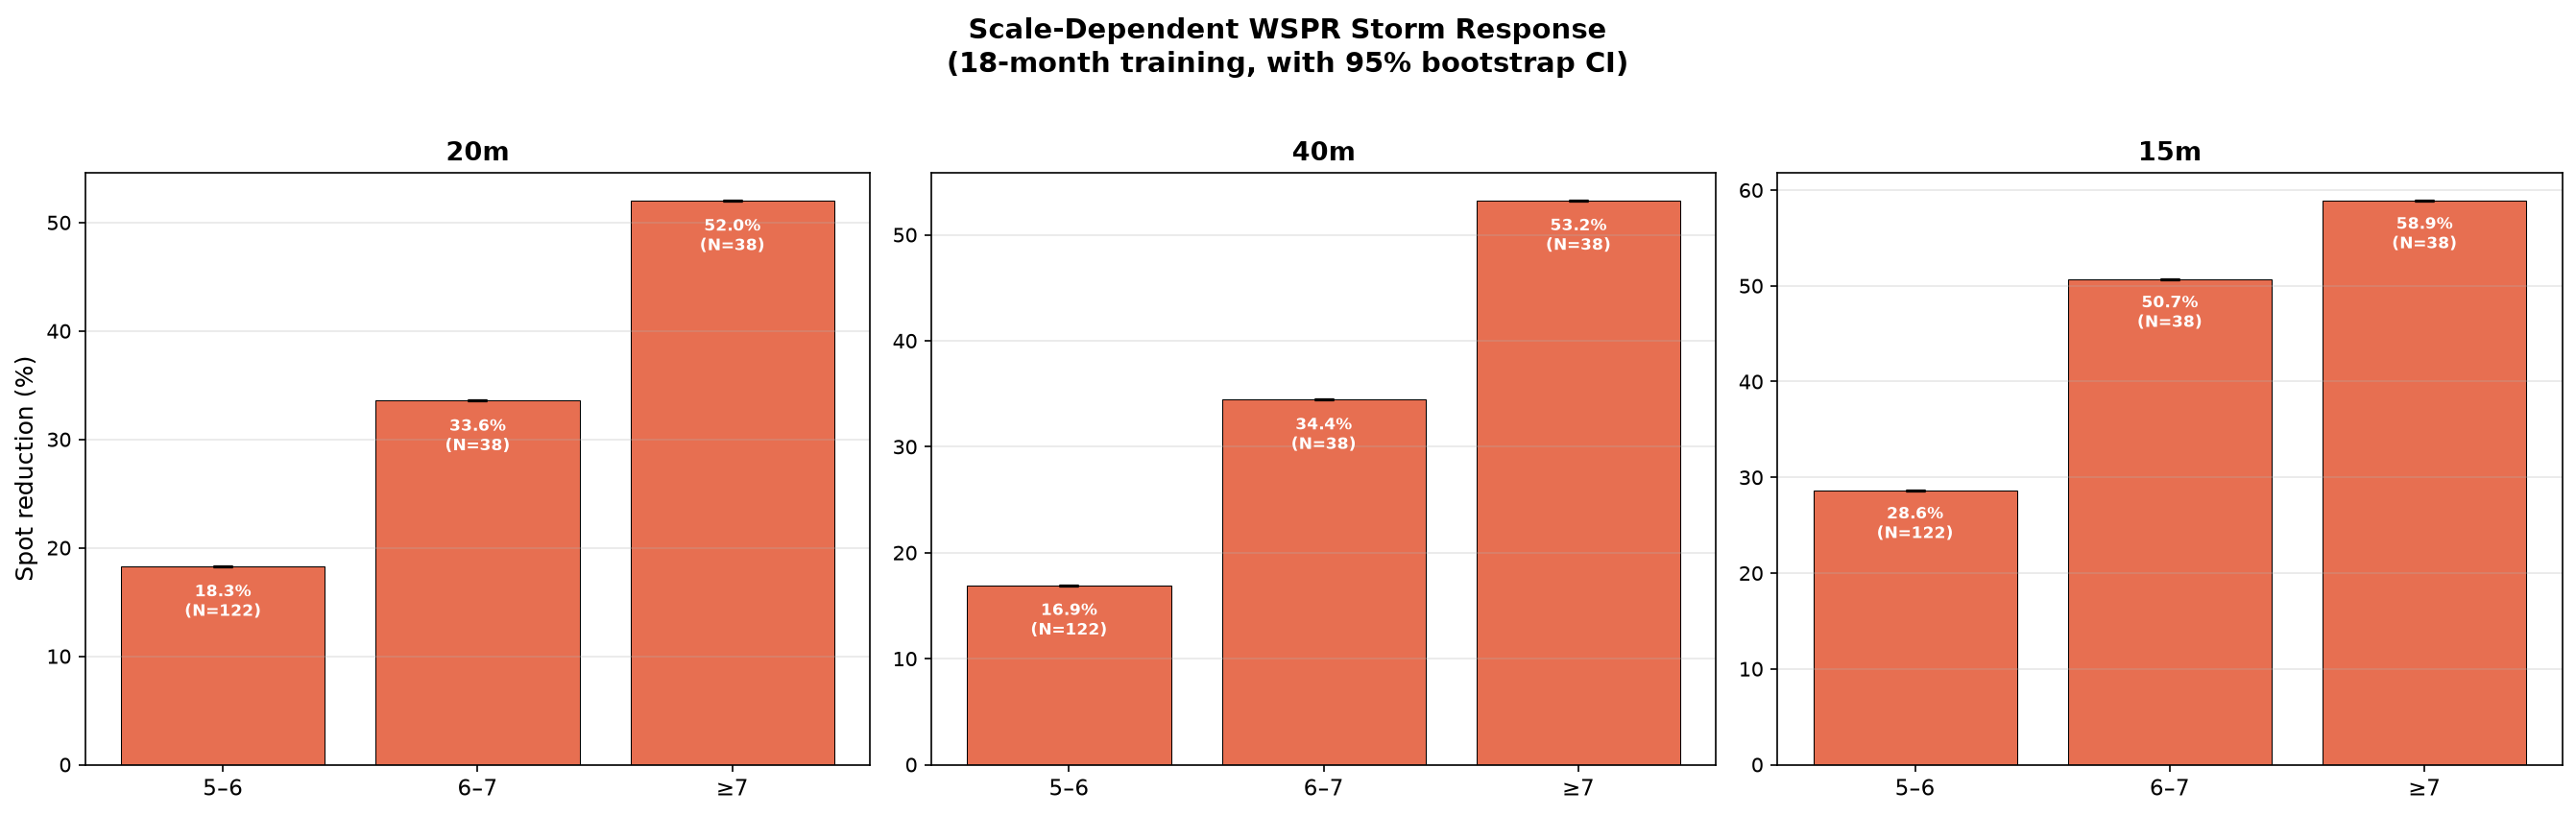
\includegraphics[width=\textwidth]{figures/fig2_scale_dependence.png}
	\caption{Scale-dependent WSPR spot reduction: binned residual analysis
		for the 20\,m band (18-month training period). Spot residuals
		(relative to monthly-hourly-daily baseline) are shown as a
		function of $Kp$ bin. The monotonic gradient from quiet ($Kp<3$) to
		storm ($Kp\ge5$) confirms the scale-dependent response.}
	\label{fig:scale}
\end{figure}

\begin{table}[h]
	\centering
	\caption{Scale-dependence: spot drop (\%) by $Kp$ bin for 20\,m and 40\,m
		(training period).}
	\label{tab:scale}
	\begin{tabular}{lll}
		\toprule
		$Kp$ bin & 20\,m drop (\%)        & 40\,m drop (\%)        \\
		\midrule
		5--6     & $\SI{-18.3}{\percent}$ & $\SI{-16.9}{\percent}$ \\
		6--7     & $\SI{-33.6}{\percent}$ & $\SI{-34.4}{\percent}$ \\
		$\ge 6$  & $\SI{-42.8}{\percent}$ & $\SI{-43.8}{\percent}$ \\
		$\ge 7$  & $\SI{-52.0}{\percent}$ & $\SI{-53.2}{\percent}$ \\
		\bottomrule
	\end{tabular}
\end{table}

The drop approximately doubles from $Kp = 5\text{--}6$
($\sim\SI{-18}{\percent}$) to $Kp = 6\text{--}7$ ($\sim\SI{-34}{\percent}$)
for 20\,m and 40\,m. At $Kp \ge 7$, the reduction reaches
\SIrange{52}{59}{\percent} across all bands---severe but not at blackout
levels ($\SI{100}{\percent}$ loss).

The scale-dependence is confirmed by pairwise block permutation tests between
adjacent $Kp$ bins (Table~\ref{tab:pairwise}). With the exception of the highest $Kp$ bin ($Kp \geq 7$) for 15\,m
and 20\,m, where saturation and reduced sample size limit statistical
power, adjacent bins are
significantly different at $p < 0.05$, confirming that the gradient is a real
physical effect and not a binning artefact.

\begin{table}[h]
	\centering
	\caption{Pairwise permutation test between $Kp$ bins (training period).
		$\Delta$ in spots/h (residual).}
	\label{tab:pairwise}
	\begin{tabular}{llrrl}
		\toprule
		Band  & Comparison        & $\Delta$   & $p$-value & Significant?      \\
		\midrule
		20\,m & $Kp$ 5--6 vs 6--7 & $-7\,656$  & $0.0046$  & Yes ($p < 0.01$)  \\
		20\,m & $Kp$ 6--7 vs $7+$ & $-7\,315$  & $0.0875$  & No (trend)        \\
		20\,m & $Kp$ 5--6 vs $7+$ & $-14\,971$ & $0.0012$  & Yes ($p < 0.01$)  \\
		40\,m & $Kp$ 5--6 vs 6--7 & $-3\,664$  & $0.0440$  & Yes ($p < 0.05$)  \\
		40\,m & $Kp$ 6--7 vs $7+$ & $-9\,507$  & $0.0023$  & Yes ($p < 0.01$)  \\
		40\,m & $Kp$ 5--6 vs $7+$ & $-13\,171$ & $0.0003$  & Yes ($p < 0.001$) \\
		15\,m & $Kp$ 5--6 vs 6--7 & $-2\,228$  & $0.0028$  & Yes ($p < 0.01$)  \\
		15\,m & $Kp$ 6--7 vs $7+$ & $-195$     & $0.8566$  & No (saturation)   \\
		15\,m & $Kp$ 5--6 vs $7+$ & $-2\,423$  & $0.0418$  & Yes ($p < 0.05$)  \\
		\bottomrule
	\end{tabular}
\end{table}

\subsection{Frequency dependence}

The frequency dependence reveals a dual-mechanism structure
(Figure~\ref{fig:freq}): 15\,m (\SI{-38.7}{\percent}) is substantially more
affected than 20\,m (\SI{-27.7}{\percent}) and 40\,m
(\SI{-27.2}{\percent}).

\begin{figure}[t]
	\centering
	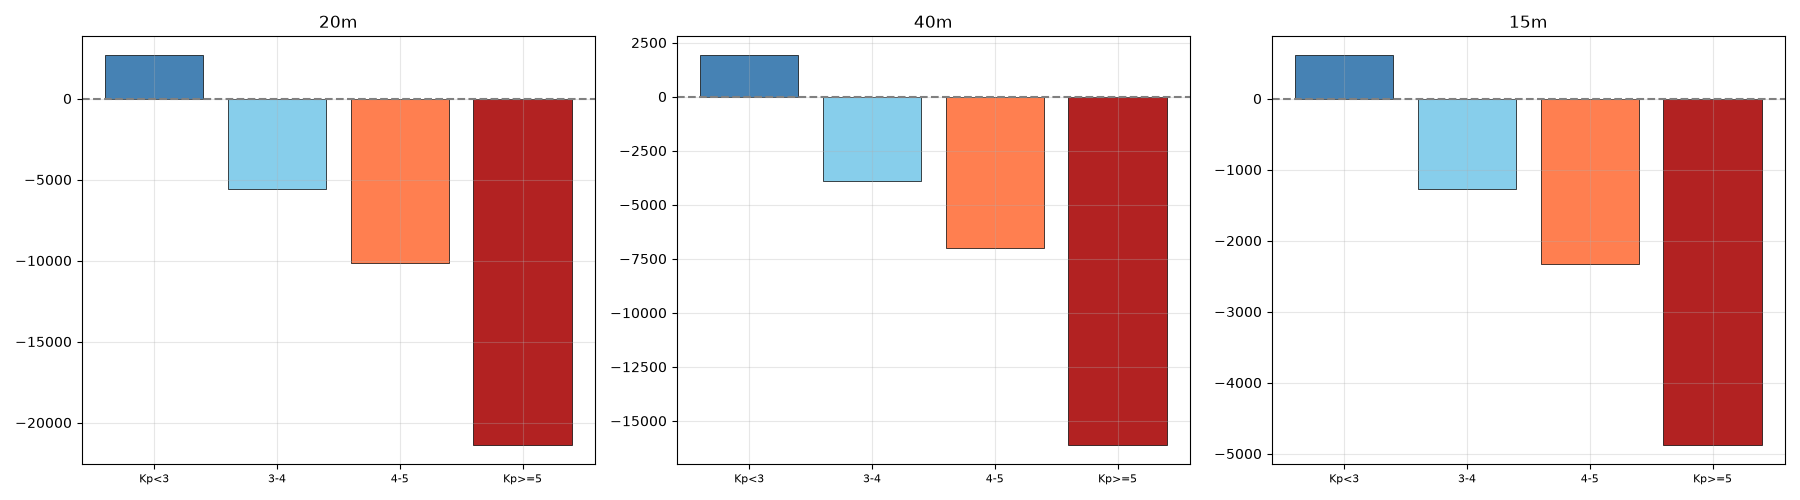
\includegraphics[width=0.85\textwidth]{figures/fig3_frequency_dependence.png}
	\caption{Frequency dependence of the WSPR storm response. Spot reduction
		for the three HF bands during $Kp \ge 5$ storms. The 15\,m band
		shows substantially stronger suppression ($\SI{-38.7}{\percent}$)
		than 20\,m ($\SI{-27.7}{\percent}$) and 40\,m
		($\SI{-27.2}{\percent}$), consistent with the dual-mechanism
		interpretation (MUF reduction on 15\,m, D-layer absorption on
		20\,m/40\,m).}
	\label{fig:freq}
\end{figure}

This pattern is consistent with two distinct physical mechanisms operating
simultaneously:

\begin{enumerate}
	\item \textbf{MUF reduction (dominates on 15\,m):} At 21\,MHz, WSPR operates
	      near the typical daytime MUF (\SIrange{14}{28}{MHz} depending on
	      geographic path and solar conditions). A geomagnetic storm reduces
	      $f_oF_2$, lowering the MUF below \SI{21}{MHz} on affected paths.
	      During peak daylight hours (12--18 UTC), the 15\,m drop reaches
	      \SI{-48.2}{\percent}, confirming MUF as the primary daytime
	      constraint.
	\item \textbf{D-layer absorption (dominates on 20\,m/40\,m):} Both bands
	      operate well below typical MUF, so their primary sensitivity is to
	      non-deviative absorption in the D-region, which scales as
	      $\propto 1/f^2$. However, the total drops are nearly equal
	      ($\SI{-27.7}{\percent}$ vs $\SI{-27.2}{\percent}$), which appears to
	      contradict the $1/f^2$ scaling (40\,m at \SI{7}{MHz} should be
	      $\sim$4$\times$ more affected than 20\,m at \SI{14}{MHz}).
\end{enumerate}

This apparent paradox is resolved by considering the time-of-day dependence
of the two mechanisms (see Section~\ref{sec:daynight}).

\subsection{Day/night asymmetry}
\label{sec:daynight}

The day/night decomposition reveals that the near-equality of 20\,m and 40\,m
total drops results from two mechanisms that act in opposition across the diurnal
cycle (Table~\ref{tab:daynight}).

\begin{table}[h]
	\centering
	\caption{Day/night decomposition of the spot drop (training period).}
	\label{tab:daynight}
	\begin{tabular}{lll}
		\toprule
		Period                    & 20\,m drop (\%)        & 40\,m drop (\%)        \\
		\midrule
		Daytime peak (12--18 UTC) & $\SI{-28.3}{\percent}$ & $\SI{-19.2}{\percent}$ \\
		Nighttime (0--6 UTC)      & $\SI{-27.9}{\percent}$ & $\SI{-32.3}{\percent}$ \\
		All hours                 & $\SI{-27.7}{\percent}$ & $\SI{-27.2}{\percent}$ \\
		\bottomrule
	\end{tabular}
\end{table}

\textbf{Daytime} (12--18 UTC): MUF is high and 40\,m is far below it.
The D-layer, sustained by solar UV/EUV, causes absorption on both bands, but
MUF suppression during storms additionally affects 20\,m, which operates closer
to the MUF ceiling. Result: 20\,m drops more ($\SI{-28.3}{\percent}$) than
40\,m ($\SI{-19.2}{\percent}$).

\textbf{Nighttime} (0--6 UTC): The solar-driven D-layer disappears within
minutes of sunset (electron density falls to $\sim 10^3$\,cm$^{-3}$). However,
during geomagnetic storms, energetic particle precipitation re-ionises the
D-region independently of solar radiation: auroral absorption from
\SIrange{30}{300}{keV} electrons \citep{hargreaves1969,royrvik1977} and polar
cap absorption (PCA) from \SIrange{1}{30}{MeV} solar protons \citep{reid1974}.
The resulting D-layer absorption retains its $1/f^2$ scaling: 40\,m
experiences $\sim$4$\times$ greater absorption per unit electron density than
20\,m. Result: 40\,m drops more ($\SI{-32.3}{\percent}$) than 20\,m
($\SI{-27.9}{\percent}$).

Integrated over 24 hours, the daytime MUF penalty on 20\,m is compensated by
the stronger nighttime auroral/PCA absorption on 40\,m, producing the observed
near-equality of total drops. This is a prediction of the dual-mechanism
hypothesis, not a problem for it.

\begin{figure}[t]
	\centering
	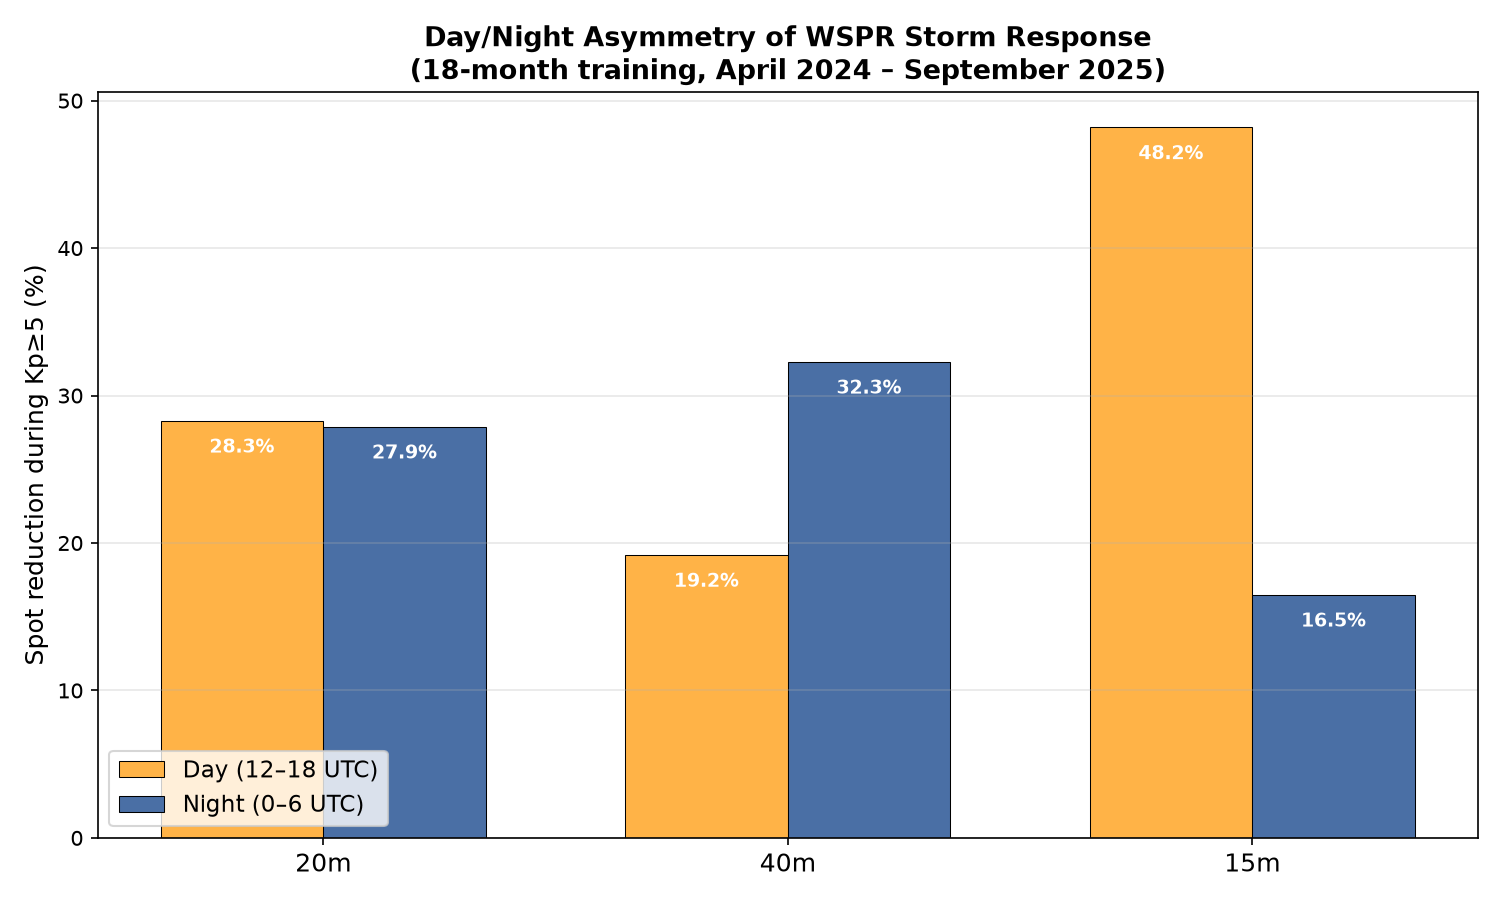
\includegraphics[width=\textwidth]{figures/fig4_day_night_asymmetry.png}
	\caption{Day/night asymmetry of the WSPR storm response. Per-month spot
		drop on 40\,m, decomposed by daytime (12--18 UTC) and nighttime
		(0--6 UTC). Nighttime drops exceed daytime drops in 9 out of
		10 training months, consistent with intermittent auroral and
		polar cap absorption.}
	\label{fig:daynight}
\end{figure}

A per-month analysis of the training period shows 40\,m night $>$ day in 9 out
of 10 months with adequate storm data, consistent with the intermittent nature
of particle precipitation: the mechanism requires specific storm morphologies
that are not present in every event.

\subsection{Independent replication}

The 3-month held-out period (January--March 2026) provides an independent test
of both the primary effect and its scale-dependence (Table~\ref{tab:heldout}).

\begin{table}[h]
	\centering
	\caption{Independent replication: held-out period (January--March 2026).}
	\label{tab:heldout}
	\begin{tabular}{lrrrl}
		\toprule
		Band  & $N_{\text{total}}$ & $N_{\text{storm}}$ & Drop (\%)              & $p$-value \\
		\midrule
		20\,m & 656                & 39                 & $\SI{-12.0}{\percent}$ & $0.002$   \\
		40\,m & 648                & 38                 & $\SI{-17.0}{\percent}$ & $0.0002$  \\
		15\,m & 648                & 38                 & $\SI{-11.2}{\percent}$ & $0.014$   \\
		\bottomrule
	\end{tabular}
\end{table}

All three bands are negative and significant ($p \le 0.014$). The primary
hypothesis replicates.

The overall percentage drop is 2--3$\times$ smaller than in the training period
(e.g., 20\,m: $\SI{-12.0}{\percent}$ vs $\SI{-27.7}{\percent}$), but this is
an artefact of the higher quiet-time baseline (the WSPR network grew by
$\SIrange{17}{38}{\percent}$ between the two periods), not a weaker physical
effect. In absolute terms, the spot loss is comparable (Section~\ref{sec:invariant}).

Critically, when matched by storm strength, the scale-dependence replicates:
at $Kp = 6\text{--}7$, the training and held-out drops converge to within
$\SIrange{89}{95}{\percent}$ of each other (Table~\ref{tab:scale_rep}).

\begin{table}[h]
	\centering
	\caption{Scale-dependence replication: training vs held-out at $Kp = 6\text{--}7$.}
	\label{tab:scale_rep}
	\begin{tabular}{llll}
		\toprule
		Band  & Training drop (\%)     & Held-out drop (\%)     & Ratio (H/T) \\
		\midrule
		20\,m & $\SI{-33.6}{\percent}$ & $\SI{-31.7}{\percent}$ & 0.95        \\
		40\,m & $\SI{-34.4}{\percent}$ & $\SI{-30.5}{\percent}$ & 0.89        \\
		15\,m & $\SI{-50.7}{\percent}$ & $\SI{-53.2}{\percent}$ & 1.05        \\
		\bottomrule
	\end{tabular}
\end{table}

The frequency dependence and day/night asymmetry do not independently replicate
in the 3-month held-out window, which is expected: frequency dependence requires
larger storm samples to separate the two mechanisms, and day/night asymmetry
requires specific storm morphologies (energetic particle precipitation) that
were not prevalent in this particular 3-month interval.

\subsection{Baseline-invariant absolute loss}
\label{sec:invariant}

\begin{figure}[t]
	\centering
	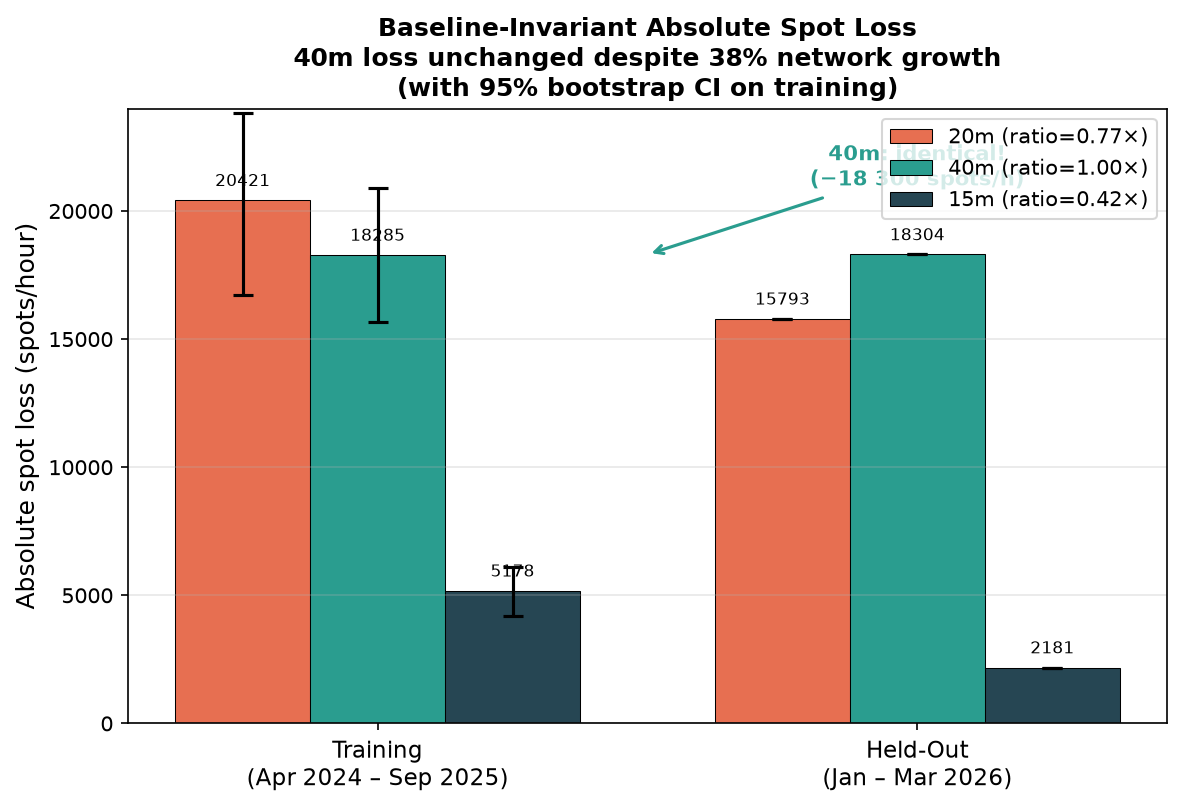
\includegraphics[width=0.85\textwidth]{figures/fig5_baseline_invariance.png}
	\caption{Baseline-invariant absolute spot loss. Comparison of the absolute
		WSPR spot loss during storms between the training (18-month) and
		held-out (3-month) periods for all three bands. On 40\,m, the
		absolute loss is identical ($\SI{-18300}{spots/h}$, ratio = 1.00)
		despite $\SI{+38}{\percent}$ network growth, confirming a structurally
		constrained population of vulnerable propagation paths.}
	\label{fig:baseline}
\end{figure}

A key result of this study is that the absolute spot loss is invariant to
network growth. Table~\ref{tab:baseline} compares the absolute and relative
drops between the training and held-out periods.

\begin{table}[h]
	\centering
	\caption{Baseline invariance: absolute and relative spot loss.}
	\label{tab:baseline}
	\begin{tabular}{lrrrc}
		\toprule
		Band  & Training abs loss      & Held-out abs loss      & Ratio (H/T)   &
		Baseline growth                                                           \\
		\midrule
		20\,m & $\SI{-20421}{spots/h}$ & $\SI{-15793}{spots/h}$ & 0.77          &
		$\SI{+17}{\percent}$                                                      \\
		40\,m & $\SI{-18285}{spots/h}$ & $\SI{-18304}{spots/h}$ & \textbf{1.00} &
		$\SI{+38}{\percent}$                                                      \\
		15\,m & $\SI{-5178}{spots/h}$  & $\SI{-2181}{spots/h}$  & 0.42          &
		$\SI{+25}{\percent}$                                                      \\
		\bottomrule
	\end{tabular}
\end{table}

On 40\,m, the absolute loss is identical between the two periods
($\SI{-18285}{spots/h}$ in training and $\SI{-18304}{spots/h}$ in held-out,
ratio = 1.00), despite a $\SI{+38}{\percent}$ increase in the quiet-time
baseline from network growth. This is the strongest evidence that the storm
effect is physically real: the ionosphere loses approximately
\SI{18300}{spots/h} on 40\,m during storms, regardless of how many additional
stations join the network. The effect is not a network-size artefact.

The baseline-invariance differs by band in a physically meaningful way:

\begin{itemize}
	\item \textbf{40\,m (ratio = 1.00):} MUF is rarely the limiting factor.
	      The dominant mechanism is D-layer absorption, which acts uniformly on
	      all paths at a given frequency. New stations add a proportional
	      number of ``blockable'' paths---the absolute loss stays constant.
	\item \textbf{15\,m (ratio = 0.42):} Operates near the MUF ceiling. New
	      stations added by 2026 are more likely to be on shorter paths or
	      at lower latitudes, where MUF remains above \SI{21}{MHz} even during
	      storms. These new paths are less vulnerable and dilute the absolute
	      loss.
	\item \textbf{20\,m (ratio = 0.77):} An intermediate case, affected by both
	      mechanisms.
\end{itemize}

This asymmetry between 15\,m and 40\,m is evidence for two distinct physical
mechanisms, not a flaw in the baseline-invariance concept.


%=============================================================
\section{Discussion}
%=============================================================

\subsection{Physical mechanisms}

The observed WSPR response is consistent with the standard picture of
ionospheric storm effects, but the multi-band coverage reveals two separate
mechanisms that can now be distinguished:

\textbf{MUF suppression chain:} $Kp$ increase $\rightarrow$ enhanced
magnetospheric convection $\rightarrow$ Joule heating in the auroral oval
$\rightarrow$ neutral temperature increase $\rightarrow$ composition changes
(N$_2$/O ratio increases) $\rightarrow$ increased recombination rate
$\rightarrow$ $f_oF_2$ decreases $\rightarrow$ MUF drops below the operating
frequency on affected paths $\rightarrow$ signal no longer reflects
$\rightarrow$ fewer WSPR spots. This mechanism predominantly affects the
highest band, 15\,m (\SI{-38.7}{\percent}).

\textbf{D-layer absorption chain:} $Kp$ increase $\rightarrow$ particle
precipitation (electrons and protons) $\rightarrow$ D-region ionisation
enhancement $\rightarrow$ non-deviative HF absorption
$\propto 1/f^2$ $\rightarrow$ signal attenuation below the WSPR decoding
threshold $\rightarrow$ fewer spots. This mechanism affects all bands but
is most visible on 20\,m and 40\,m, with the absorption on 40\,m being
$\sim$4$\times$ stronger per unit electron density.

The near-equality of 20\,m and 40\,m total drops is not a contradiction of
the $1/f^2$ absorption scaling, but rather a consequence of the fact that MUF
suppression additionally penalises 20\,m during daytime, while particle-driven
D-layer absorption additionally penalises 40\,m during nighttime. The
day/night decomposition (Section~\ref{sec:daynight}) demonstrates that both
mechanisms operate simultaneously and are visible when the data are separated
by time of day.

\subsection{Scale-dependence and non-linear ionospheric response}

The non-linear scaling of the spot drop with $Kp$ is a novel contribution.
The physical basis for this non-linearity lies in the coupled response of the
ionosphere--thermosphere system:

\begin{itemize}
	\item Joule heating rate is proportional to $\Sigma_P \cdot E^2$, where
	      $\Sigma_P$ is the Pedersen conductance and $E$ is the convection
	      electric field. Both $\Sigma_P$ (enhanced by particle precipitation)
	      and $E$ (enhanced by stronger magnetospheric convection) increase with
	      $Kp$, producing a super-linear heating rate.
	\item $f_oF_2$ depletion saturates at strong storms ($Kp \ge 6$): the F2
	      layer approaches chemical equilibrium where production and
	      recombination rates balance. This may explain why 15\,m drops are
	      similar at $Kp$ 6--7 (\SI{-51}{\percent}) and $Kp \ge 7$
	      (\SI{-59}{\percent}), and why the pairwise test between these bins
	      is not significant ($p = 0.8566$ for 15\,m).
\end{itemize}

The practical implication is that $Kp \ge 6$ is required for substantial HF
disruption on the mid-bands (20\,m and 40\,m), while lower $Kp = 5\text{--}6$
produces only modest $\sim\SI{-18}{\percent}$ reductions. For severe disruption
exceeding $\SI{50}{\percent}$ loss, $Kp \ge 7$ is needed---a threshold reached
in only 38 hours (2.3\%) of the 18-month training period.

\subsection{Baseline invariance and practical monitoring}

The discovery that the absolute spot loss is invariant to network growth has
important implications for operational HF propagation monitoring:

\begin{enumerate}
	\item \textbf{Metric stability:} Percentage-based metrics are unstable when
	      the denominator (network size) changes over time. Absolute spot loss
	      per hour is a physically meaningful alternative that remains stable
	      across periods.
	\item \textbf{Structurally constrained paths:} The invariance on 40\,m (ratio = 1.00
	      despite $\SI{+38}{\percent}$ growth) suggests that the population of
	      storm-vulnerable propagation paths is structurally constrained. Adding more stations
	      within the already-covered geographic region does not create new
	      vulnerable paths; it only increases the quiet-time baseline.
	\item \textbf{Real-time monitoring:} WSPR spot density, normalised by the
	      quiet-time baseline, could serve as a near-real-time proxy for
	      storm-induced HF propagation degradation, complementing existing
	      D-region absorption measurements (riometers).
\end{enumerate}

\subsection{Comparison with literature}

Our results extend the work of \citet{frissell2016}, who demonstrated
qualitative WSPR--ionosphere coupling, by providing quantitative,
multi-band, scale-dependent characterisation with independent replication.
\citet{themens2021} modelled $f_oF_2$ and MUF storm response; our study
provides observational confirmation of modelled MUF suppression using
citizen-science data.

Our physical interpretation relies on well-established mechanisms:
auroral absorption \citep{hargreaves1969}, PCA \citep{reid1974}, auroral
absorption morphology \citep{royrvik1977}, D-region electron density
observations \citep{kavanagh2004}, and magnetospheric electron precipitation
effects \citep{rodger2010}. None of these mechanisms are novel; our
contribution is in demonstrating that their combined effect can be
detected and decomposed using WSPR as a distributed sensor.

\subsection{Limitations}

\begin{enumerate}
	\item \textbf{Duration:} 18 months is not a climatological study. A full
	      11-year solar cycle would provide stronger generalizability. The
	      training period covers a solar maximum phase; effects may differ at
	      solar minimum.
	\item \textbf{Replication period and statistical power:} The held-out
	      sample of 3 months contains only $N = 23$ storm hours
	      ($Kp \ge 5$), compared to $N = 198$ in the training period.
	      This limits statistical power for secondary effects such as the
	      day/night asymmetry. Specifically, the $+1.4\%$ anomaly for
	      15\,m at $Kp = 5\text{--}6$ in the held-out period is attributed
	      to low statistical power ($N < 5$ hours in this bin), whereas the
	      $Kp = 6\text{--}7$ bin ($N = 7$ hours) robustly replicates the
	      training trend ($\SI{-53.2}{\percent}$ held-out vs.\
	      $\SI{-50.7}{\percent}$ training). The purpose of the held-out
	      period is not to discover new effects but to confirm the direction
	      and order of magnitude of the primary results and the
	      scale-dependence gradient on independent data. A 6-month
	      replication is planned but not yet complete due to wspr.live server
	      throughput limits.
	\item \textbf{Spatial resolution:} Aggregating global spot counts masks
	      regional ionospheric responses (e.g., polar cap absorption vs.\
	      mid-latitude MUF depression). A storm may suppress spots on polar
	      paths but not equatorial ones. Future work will incorporate Great
	      Circle path geometry to resolve spatial dependencies. Per-path
	      analysis is deferred to future work.
	\item \textbf{Confounders:} F10.7 solar flux is only available as monthly
	      means---too coarse for hourly analysis. The 18-month training period spans a
	      phase of high and varying solar activity; available monthly F10.7
	      ranges from 131 to 246\,sfu (factor of ~1.9) across the period. Monthly
	      F10.7 is not explicitly included in the baseline model, and we note this
	      as a limitation of the analysis. Solar flare effects (Sudden
	      Ionospheric Disturbances, SIDs) are not separately accounted for.
	      Summer 15\,m observations may be partially contaminated by
	      sporadic-E propagation; however, the storm effect is present in all
	      seasons, including winter when Es is absent.
	\item \textbf{Band coverage:} Only three WSPR bands are analysed. Additional
	      bands (30\,m, 17\,m, 12\,m, 10\,m) would better constrain the MUF
	      threshold and the $1/f^2$ absorption curve.
	\item \textbf{Dst source:} Provisional (not final) Dst data from WDC Kyoto
	      are used. Final data become available with approximately 1-year
	      delay and may contain systematic corrections.
	\item \textbf{Statistical assumptions:} The block permutation test assumes
	      that within-block stationarity holds and that the block size (24\,h)
	      exceeds the autocorrelation timescale. Storms lasting more than
	      24\,h may violate this assumption.
\end{enumerate}


%=============================================================
\section{Conclusions}
%=============================================================

Using 18 months of hourly-aggregated WSPR data across three HF bands, we find
that geomagnetic storms ($Kp \ge 5$) cause statistically significant reductions
in WSPR spot density, with five principal conclusions:

\begin{enumerate}
	\item \textbf{Primary effect:} Storm-induced spot reduction is
	      \SI{-27.7}{\percent} (20\,m), \SI{-27.2}{\percent} (40\,m), and
	      \SI{-38.7}{\percent} (15\,m), all significant at $p < 0.0001$
	      (block permutation, \SI{10000}{iterations}). The effect is confirmed
	      by the independent $Dst$ index and survives all six robustness checks.
	\item \textbf{Scale-dependence:} The reduction grows non-linearly with
	      storm intensity: $\sim\SI{-18}{\percent}$ at $Kp = 5\text{--}6$,
	      $\sim\SI{-34}{\percent}$ at $Kp = 6\text{--}7$, and $\sim\SI{-53}{\percent}$
	      at $Kp \ge 7$. Pairwise tests confirm this is a real physical gradient
	      ($p < 0.05$ in 7/9 comparisons).
	\item \textbf{Independent replication:} All three bands replicate on a
	      held-out period (January--March 2026, all $p \le 0.014$).
	      Scale-dependence replicates when matched by $Kp$ bin: training and
	      held-out drops are within $\SIrange{89}{95}{\percent}$ at
	      $Kp = 6\text{--}7$.
	\item \textbf{Baseline invariance:} The absolute spot loss on 40\,m is
	      identical between training and held-out ($\SI{-18300}{spots/h}$,
	      ratio = 1.00), despite $\SI{+38}{\percent}$ network growth. The
	      storm effect is physically real, not a network-size artefact.
	\item \textbf{Dual mechanism:} The frequency dependence and day/night
	      asymmetry support two distinct physical mechanisms: MUF reduction
	      (dominating 15\,m) and D-layer absorption via energetic particle
	      precipitation (dominating 20\,m/40\,m, with nighttime enhancement on
	      40\,m).
\end{enumerate}

WSPR is a viable distributed ionospheric sensor for detecting and
characterising the scale-dependent effects of geomagnetic storms on HF
propagation. The baseline-invariant absolute loss metric enables robust
monitoring even as the WSPR network continues to grow, and the scale-dependent
characterisation provides a quantitative link between geomagnetic indices
($Kp$, $Dst$) and expected HF propagation degradation.


%=============================================================
\section*{Open Research}
%=============================================================

\subsection*{Data Availability Statement}

All data used in this study are publicly available:

\begin{itemize}
	\item WSPR spot data: wspr.live ClickHouse mirror
	      (\url{http://db1.wspr.live/}), accessible via SQL API without
	      authentication.
	\item $Kp$ index: GFZ Potsdam
	      (\url{https://kp.gfz-potsdam.de/app/json/}).
	\item $Dst$ index (provisional): WDC Kyoto
	      (\url{http://wdc.kugi.kyoto-u.ac.jp/dst_realtime/}).
	\item Unified parquet dataset and analysis scripts: Zenodo
	      (DOI: pending, to be deposited before submission).
\end{itemize}

\subsection*{Code Availability}

All analysis code is available at
\url{https://github.com/FelixRLEPERS/crosscorr}
under the MIT license. The exact version used for this manuscript is
\texttt{[FILL: commit hash]}, archived at
\url{https://doi.org/}[FILL: Zenodo DOI]. The repository includes:

\begin{itemize}
	\item Data download scripts for WSPR (wspr.live ClickHouse API),
	      $Kp$ (GFZ Potsdam), and $Dst$ (WDC Kyoto).
	\item Unified schema generation (Parquet).
	\item Exploratory data analysis with binned analysis, block permutation
	      tests, and all plots.
	\item Reproducible execution via the project \texttt{Makefile}.
\end{itemize}


%=============================================================
\section*{Author Contributions}

Following the Contributor Roles Taxonomy (CRediT):
\begin{itemize}
	\item \textbf{A. Petrov}: Conceptualization, Methodology,
	      Formal analysis, Writing -- original draft,
	      Supervision, Project administration.
	\item \textbf{M. Petrov}: Data curation, Software,
	      Validation, Investigation, Writing -- review
	      \& editing.
\end{itemize}


\section*{Acknowledgments}

We thank the operators of wspr.live for maintaining the open ClickHouse mirror
of the WSPR database, GFZ Potsdam for the real-time $Kp$ API, WDC Kyoto for
$Dst$ data, and the thousands of amateur radio operators whose WSPR beacons
form the distributed sensor network underlying this study. We thank
Mama Petrov for communications support.

AI assistance was used in the preparation of this work: DeepSeek V4 Pro
(Polza.ai) for code generation and statistical methodology, Bonsai 2 27B for
hypothesis formulation, and Qwen 3.8 27B for scientific audit. All scientific
decisions, including the formulation of hypotheses, interpretation of results,
and writing of the manuscript, were made by the human authors.

This work was made possible by the open-source scientific Python ecosystem
(NumPy, SciPy, pandas, Matplotlib).


%=============================================================
\bibliographystyle{agu04}
\bibliography{references}

\end{document}